\chapter{Option pricing}

\section{Prix du Call européen dans le modèle de Black-Scholes}

\begin{exerciseBox}[Prix du Call européen dans le modèle de Black-Scholes]
Soit un actif \( S_t \) évoluant selon la dynamique :
\[
dS_t = r S_t\, dt + \sigma S_t\, dW_t
\]

où \( r \) est le taux sans risque constant, \( \sigma > 0 \), et \( (W_t) \) est un mouvement brownien sous la mesure risque-neutre.

\vspace{1cm}

On considère une option Call européenne de maturité \( T \) et de strike \( K \). 

\vspace{1cm}

\textbf{Question :} Montrer que le prix \( C_0 \) du Call à \( t=0 \) est donné par :
\[
C_0 = S_0 \Phi(d_1) - K e^{-rT} \Phi(d_2)
\]

avec :
\[
d_1 = \frac{\ln(S_0/K) + (r + \frac{\sigma^2}{2})T}{\sigma \sqrt{T}}, 
\quad 
d_2 = d_1 - \sigma \sqrt{T}
\]
\end{exerciseBox}


\section*{Solution :}

Sous la mesure risque-neutre \( \mathbb{Q} \), l’actif sous-jacent suit :

\[
dS_t = r S_t\, dt + \sigma S_t\, dW_t^{\mathbb{Q}}, \quad S_0 > 0
\]

La solution de cette EDS est :

\[
S_T = S_0 \cdot \exp\left( \left(r - \frac{\sigma^2}{2}\right)T + \sigma W_T^{\mathbb{Q}} \right)
\]

Le prix du call européen à \( t = 0 \) est donné par :

\[
C_0 = e^{-rT} \cdot \mathbb{E}^{\mathbb{Q}}\left[ (S_T - K)_+ \right]
\]


\subsection*{Décomposition de l’espérance}

\[
(S_T - K)_+ = S_T \cdot \mathbf{1}_{S_T > K} - K \cdot \mathbf{1}_{S_T > K}
\]

\[
\Rightarrow C_0 = e^{-rT} \left( \mathbb{E}[S_T \cdot \mathbf{1}_{S_T > K}] - K \cdot \mathbb{E}[ \mathbf{1}_{S_T > K}] \right)
\]


\subsection*{1. Calcul de \( \mathbb{E}[ \mathbf{1}_{S_T > K}] \)}

On a :


\begin{align*}
\mathbb{P}(S_T > K) 
&= \mathbb{P}\left( \ln\left( \frac{S_T}{K} \right) > 0 \right) 
\quad \text{(\(\ln\) est croissante)} \\
&= \mathbb{P}\left( \ln(S_T) > \ln(K) \right) \\
&= \mathbb{P}\left( \ln(S_0) + \left(r - \frac{\sigma^2}{2}\right)T + \sigma W_T^{\mathbb{Q}} > \ln(K) \right) 
 \\
&= \mathbb{P}\left( \sigma W_T^{\mathbb{Q}} > \ln(K) - \ln(S_0) - \left(r - \frac{\sigma^2}{2}\right)T \right) \\
&= \mathbb{P}\left( W_T^{\mathbb{Q}} > \frac{1}{\sigma} \left[ \ln(K/S_0) - \left(r - \frac{\sigma^2}{2}\right)T \right] \right) \\
&= \mathbb{P}\left( W_T^{\mathbb{Q}} > -d_2 \cdot \sqrt{T} \right) 
\quad \text{(on pose \( d_2 := \frac{\ln(S_0/K) + (r - \frac{\sigma^2}{2})T}{\sigma \sqrt{T}} \))} \\
&= \mathbb{P}\left( \frac{W_T^{\mathbb{Q}}}{\sqrt{T}} > -d_2 \right) 
\quad \text{(car \( W_T^{\mathbb{Q}} \sim \mathcal{N}(0, T) \))} \\
&= \mathbb{P}(G > -d_2), \quad G \sim \mathcal{N}(0,1) \\
&= 1 - \Phi(-d_2) \quad \text{avec $\Phi$ est la F.D.R du loi $\mathcal{N}(0,1)$} \\
&= \Phi(d_2) , \quad \Phi(-x) + \Phi(x) = 1
\end{align*}

% \newpage

\subsection*{2. Calcul de \( \mathbb{E}[S_T \cdot \mathbf{1}_{S_T > K}] \)}

\begin{rappelBox}[Théorème de Girsanov]
Soit \( (W_t)_{t \geq 0} \) un mouvement brownien sous \( \mathbb{P} \), et \( (h_t)_{t \geq 0} \) un processus progressif, tel que :
\[
Z_t := \exp\left( -\int_0^t h_s\, dW_s - \frac{1}{2} \int_0^t h_s^2\, ds \right)
\]
soit une \( \mathbb{P} \)-martingale.

Alors, la mesure \( \mathbb{Q} \) définie par \( \left. \frac{d\mathbb{Q}}{d\mathbb{P}} \right|_{\mathcal{F}_t} = Z_t \) transforme :
\[
\widetilde{W}_t := W_t + \int_0^t h_s\, ds
\quad \text{en un Brownien sous } \mathbb{Q}.
\]
\end{rappelBox}

\textbf{Formellement}, posons :



\begin{align*}
\mathbb{E}[S_T \cdot \mathbf{1}_{S_T > K}] 
&= \mathbb{E}^{\mathbb{Q}}\left[S_0 \cdot \exp\left( \left(r - \frac{\sigma^2}{2}\right)T + \sigma W_T^{\mathbb{Q}} \right) \cdot \mathbf{1}_{S_T > K} \right] \\
&= S_0 \cdot e^{rT} \cdot \mathbb{E}^{\mathbb{Q}}\left[ \exp\left( \sigma W_T^{\mathbb{Q}} - \frac{\sigma^2}{2}T \right) \cdot \mathbf{1}_{S_T > K} \right] \\
&= S_0 \cdot e^{rT} \cdot \mathbb{E}^{\mathbb{Q}}\left[ Z_T \cdot \mathbf{1}_{S_T > K} \right]
\quad \text{avec } Z_T := \exp\left( \sigma W_T^{\mathbb{Q}} - \frac{1}{2}\sigma^2 T \right) \\
&= S_0 \cdot e^{rT} \cdot \mathbb{E}^{\mathbb{Q}}\left[ \frac{d\mathbb{P}}{d\mathbb{Q}} \cdot \mathbf{1}_{S_T > K} \right]
\quad \text{(remarque : Girsanov avec } h_t = \sigma) \\
&= S_0 \cdot e^{rT} \cdot \mathbb{P}(S_T > K) \quad \text{car} \; \mathbb{E}^{\mathbb{Q}}\left[\frac{d\mathbb{P}}{d\mathbb{Q}}Y\right] = \mathbb{E}^{\mathbb{P}}(Y) \\
&= S_0 \cdot e^{rT} \cdot \mathbb{P}\left( \ln(S_T/K) > 0 \right) \\
&= S_0 \cdot e^{rT} \cdot \mathbb{P}\left( \ln(S_T) > \ln(K) \right) \\
&= S_0 \cdot e^{rT} \cdot \mathbb{P}\left( \ln(S_0) + \left(r - \frac{\sigma^2}{2} \right)T + \sigma W_T^{\mathbb{Q}} > \ln(K) \right) \\
&= S_0 \cdot e^{rT} \cdot \mathbb{P}\left( W_T^{\mathbb{Q}} > \frac{ \ln(K/S_0) - \left(r - \frac{\sigma^2}{2} \right)T }{\sigma} \right) \\
&= S_0 \cdot e^{rT} \cdot \mathbb{P}\left( W_T^{\mathbb{Q}} - \sigma T > \frac{ \ln(K/S_0) - \left(r - \frac{\sigma^2}{2} \right)T }{\sigma} - \sigma T \right) \\
&= S_0 \cdot e^{rT} \cdot \mathbb{P}\left( W_T^{\mathbb{Q}} - \sigma T > \frac{ \ln(K/S_0) - \left(r + \frac{\sigma^2}{2} \right)T }{\sigma} \right)  \quad \text{or} \; W_T^{\mathbb{Q}} - \sigma T \sim \mathcal{N}(0,T) \; \text{sous} \; \mathbb{P} \\
&= S_0 \cdot e^{rT} \cdot \mathbb{P}\left( \frac{W_T^{\mathbb{Q}} - \sigma T}{\sqrt{T}} > -d_1 \right)
\quad \text{(on pose \( d_1 := \frac{\ln(S_0/K) + (r + \frac{\sigma^2}{2})T}{\sigma \sqrt{T}} \))} \\
&= S_0 \cdot e^{rT} \cdot \mathbb{P}(G > -d_1), \quad \text{où } G \sim \mathcal{N}(0, 1) \\
&= S_0 \cdot e^{rT} \cdot \Phi(d_1)
\end{align*}


\subsection*{Conclusion}

On obtient :

\[
C_0 = e^{-rT} \left( S_0. e^{rT} \cdot \Phi(d_1) - K \cdot \Phi(d_2) \right)
= \boxed{ S_0 \Phi(d_1) - K e^{-rT} \Phi(d_2) }
\]

avec :
\[
d_1 = \frac{\ln(S_0/K) + (r + \frac{\sigma^2}{2})T}{\sigma \sqrt{T}}, \quad
d_2 = d_1 - \sigma \sqrt{T}
\]



\section{Option Chooser}

\subsection*{Exercice :}

\begin{exerciseBox}[Option Chooser]
On considère une option \emph{chooser} définie comme suit : 
à la date $T_1$, le détenteur choisit si l’option devient un call européen ou un put européen.
L’option choisie porte sur le même actif sous-jacent $S_t$, avec la même maturité finale $T_2 > T_1$ et le même prix d’exercice $K$.

\paragraph{Question :} 
Donner le prix de cette option à $t=0$ dans le modèle de Black--Scholes.    
\end{exerciseBox}


\subsection*{Solution :}
À la date $T_1$, la valeur de l’option chooser est
\[
V(T_1) = \max \Big( C_{T_1}(K,T_2), \; P_{T_1}(K,T_2) \Big),
\]
où $C_{T_1}(K,T_2)$ et $P_{T_1}(K,T_2)$ désignent respectivement le prix d’un call et d’un put européens de strike $K$ et échéance $T_2$, évalués à la date $T_1$.

D’après la parité call--put,
\[
C_{T_1}(K,T_2) - P_{T_1}(K,T_2) = S_{T_1} - K e^{-r(T_2-T_1)}.
\]

or 
\[
\max(x,y) = y + \max(x - y , 0)
\]

Ainsi,

\begin{align*}
\max(C_{T_1},P_{T_1}) &= P_{T_1}(K , T_2) + \max(C_{T_1}(K,T_2) - P_{T_1}(K,T_2),0)\\
&= P_{T_1}(K,T_2) + \max\Big(S_{T_1} - K e^{-r(T_2-T_1)} , 0 \Big) \\
&= P_{T_1}(K,T_2) + \max\Big(S_{T_1} - K' , 0 \Big) \quad avec \; \; K'= K e^{-r(T_2-T_1)}
\end{align*}


or 
$\max\Big(S_{T_1} - K e^{-r(T_2-T_1)} , 0 \Big)$ est le payoff d'une option call de strike $K' = K e^{-r(T_2-T_1)}$ et d'échéance $T_1$

Par conséquent, le prix de l’option chooser à $t=0$ s’écrit
\[
V(0) = P(0;K,T_2) + C_0\big(K e^{-r(T_2-T_1)},T_1\big),
\]
c’est-à-dire la somme :
\begin{itemize}
    \item d’un put européen de strike $K$ et maturité $T_2$, 
    \item plus d’un call européen de strike $K e^{-r(T_2-T_1)}$ et maturité $T_1$.
\end{itemize}



\section{Option d'échange avec devise}

\subsection*{Exercice :}

\begin{exerciseBox}[Option d'échange avec devise]
Soient $Z_t$ (actif en EUR), $Y_t$ (actif en USD) et $X_t$ (taux de change EUR/USD). \\ 
soit une option de payoff à maturité $T$ est 
\[
\Pi_T=(Z_T - X_T Y_T)^+.
\]
Dans le monde de Black–Scholes  donner le prix de l'option à t= 0 ? 
\end{exerciseBox}


\subsection*{Solution}

% On travaille dans Black--Scholes avec taux constants $r^{\EUR}$ (euro) et $r^{\USD}$ (dollar).
% On note $B_t^{\EUR}=e^{r^{\EUR} t}$ et $B_t^{\USD}=e^{r^{\USD} t}$.
% Soit $W_t=(W_t^{(1)},W_t^{(2)},W_t^{(3)})$ un mouvement brownien \emph{vectoriel} sous la mesure
% domestique $\,\mathbb{Q}^{\EUR}\,$, de matrice de corrélation
% $\rho_{ij}=\mathrm{Corr}(dW^{(i)}_t,dW^{(j)}_t)$.

% Sous $\mathbb{Q}^{\EUR}$, les dynamiques risque-neutres (drifts domestiques corrects) sont
% \begin{align*}
% \frac{dZ_t}{Z_t} &= r^{\EUR}\,dt + \sigma_Z\,dW_t^{(1)},\\
% \frac{dY_t}{Y_t} &= r^{\USD}\,dt + \sigma_Y\,dW_t^{(2)},\\
% \frac{dX_t}{X_t} &= (r^{\USD}-r^{\EUR})\,dt + \sigma_X\,dW_t^{(3)}.
% \end{align*}

Le payoff vaut $(Z_T - X_T Y_T)^+$ et le prix initial est
\begin{align*}
C_0
  &= \mathbb{E}^{\mathbb{Q}^{\EUR}}\!\Big[e^{-r^{\EUR}T}\,\big(Z_T - X_TY_T\big)^+\Big]\\
  &= \mathbb{E}^{\mathbb{Q}^{\EUR}}\!\Big[e^{-r^{\EUR}T} Z_T\,\mathbf{1}_{\{Z_T\ge X_TY_T\}}\Big]
   - \mathbb{E}^{\mathbb{Q}^{\EUR}}\!\Big[e^{-r^{\EUR}T} X_TY_T\,\mathbf{1}_{\{Z_T\ge X_TY_T\}}\Big].
\end{align*}


\begin{rappelBox}[Changement de numéraire]
\begin{itemize}
    \item  Soit $(\mathbb{Q}^{\alpha},\alpha_t)$ une mesure de probabilité et un numéraire de référence,
c'est-à-dire que pour tout actif $Z_t$ ne versant pas de dividendes,
le processus $\displaystyle \frac{Z_t}{\alpha_t}$ est une $\mathbb{Q}^{\alpha}$-martingale.

\item  Soit $(\beta_t)$ un \emph{numéraire simple}, c'est-à-dire un processus strictement positif
tel que $\displaystyle \big( \frac{\beta_t}{\alpha_t} \big)_t$  soit une $\mathbb{Q}^{\alpha}$-martingale.

\end{itemize}


Alors :

\begin{enumerate}[label=\roman*)]
\item Il existe une mesure $\mathbb{Q}^{\beta}$ équivalente à $\mathbb{Q}^{\alpha}$ telle que
\[
\left.\frac{d\mathbb{Q}^{\beta}}{d\mathbb{Q}^{\alpha}}\right|_{\mathcal{F}_t}
= \frac{\alpha_0}{\alpha_t}\,\frac{\beta_t}{\beta_0}.
\]
De plus, pour tout $F_T$ v.a,
\[
\mathbb{E}^{\mathbb{Q}^{\alpha}}\!\left[
\frac{\alpha_t}{\alpha_T} F_T \,\bigg|\, \mathcal{F}_t
\right]
=
\mathbb{E}^{\mathbb{Q}^{\beta}}\!\left[
\frac{\beta_t}{\beta_T} F_T \,\bigg|\, \mathcal{F}_t
\right].
\]

\item Si $\displaystyle \frac{Z_t}{\alpha_t}$ est une $\mathbb{Q}^{\alpha}$-martingale,
alors $\displaystyle \frac{Z_t}{\beta_t}$ est une $\mathbb{Q}^{\beta}$-martingale.

\end{enumerate}
\end{rappelBox}


\paragraph{Changement de numéraire $Z$.}
Définissons la mesure $\mathbb{Q}^{Z}$ par
\[
\frac{d\mathbb{Q}^{Z}}{d\mathbb{Q}^{\EUR}}\Big|_{\mathcal{F}_T}
=\frac{e^{-r^{\EUR}T}Z_T}{Z_0}.
\]
Alors
\begin{align*}
\mathbb{E}^{\mathbb{Q}^{\EUR}}\!\Big[e^{-r^{\EUR}T} Z_T\,\mathbf{1}_{\{Z_T\ge X_TY_T\}}\Big] 
&= \mathbb{E}^{\mathbb{Q}^Z}\!\Big[\frac{Z_0}{Z_T}Z_T \mathbf{1}_{\{Z_T\ge X_TY_T\}}\Big] \\
&= Z_0\mathbb{E}^{\mathbb{Q}^Z}\!\Big[\mathbf{1}_{\{Z_T\ge X_TY_T\}}\Big] \\
&= Z_0\,\mathbb{Q}^{Z}\!\big(Z_T\ge X_TY_T\big) \\
&= Z_0\,\mathbb{Q}^{Z}\!\big( \frac{X_TY_T}{Z_T} \le 1 \big) \\
% &= Z_0\,\mathcal{N}(d_1),
\end{align*}

\textbf{loi du} $\frac{X_TY_T}{Z_T}$ sous $\mathbb{Q}^Z$ :



Comme $Z_t$ est choisi comme numéraire, donc sous la  mesure $\mathbb{Q}^Z$ on  a que  $\big(\frac{X_t Y_t}{Z_t} \big)_t$ est une martingale.

Donc : 

\begin{align*}
d\!\left( \frac{X_t Y_t}{Z_t} \right)
&= \frac{X_t Y_t}{Z_t}
   \left[ \bigl(\sigma_X + \sigma_Y - \sigma_Z \bigr)\cdot dW_t^{Z} \right],
\end{align*}
où $W_t^{Z}$ est un mouvement brownien sous $\mathbb{Q}^Z$
et le drift est nul (martingale).

On en déduit que le processus est une exponentielle stochastique :
\begin{align*}
\frac{X_t Y_t}{Z_t}
&= \frac{X_0 Y_0}{Z_0}
   \exp\!\left\{
      \bigl(\sigma_X + \sigma_Y - \sigma_Z \bigr)\cdot W_t^{Z}
      - \tfrac12
        \bigl\|\sigma_X + \sigma_Y - \sigma_Z\bigr\|^2 t
   \right\}.
\end{align*}

Soit 
\[
\sigma := \sigma_X + \sigma_Y - \sigma_Z
\quad\text{et}\quad
\hat{\sigma} := \|\sigma\|
\]
% la volatilité effective (en norme euclidienne) du ratio
% \(\displaystyle \frac{X_t Y_t}{Z_t}\)
% sous la mesure \(\mathbb{Q}^Z\).
Alors
% \[
% \mathbb{Q}^Z\!\left(\frac{X_T Y_T}{Z_T}\le 1\right)
% = \Phi\!\left(
% \frac{ \ln\!\big(\tfrac{Z_0}{X_0 Y_0}\big)
%       + \tfrac12 \hat{\sigma}^2 T }
%      { \hat{\sigma}\sqrt{T} }
% \right),
% \]


\begin{align*}
\mathbb{Q}^{Z}\!\left(\frac{X_TY_T}{Z_T}\le 1\right)
&= \mathbb{Q}^{Z}\!\left(\ln\!\frac{X_TY_T}{Z_T}\le 0\right) \\
&= \Phi\!\left(\frac{\,0-\Big(\ln\!\frac{X_0Y_0}{Z_0}-\tfrac12\hat{\sigma}^2T\Big)}{\hat{\sigma}\sqrt{T}}\right)\quad \big( \text{on a} \; \sigma.W^Z_T = \hat{\sigma} \sqrt{T} G \; \; \text{avec} \; G \sim \mathcal{N}(0,1) \big) \\
&= \Phi\!\left(\frac{\ln\!\big(\tfrac{Z_0}{X_0Y_0}\big)+\tfrac12\hat{\sigma}^2T}{\hat{\sigma}\sqrt{T}}\right).
\end{align*}

où \(\Phi\) désigne la fonction de répartition de la loi normale standard \(\mathcal{N}(0,1)\).

Donc : 

\[
\boxed{
\mathbb{E}^{\mathbb{Q}^{\EUR}}\!\Big[e^{-r^{\EUR}T} Z_T\,\mathbf{1}_{\{Z_T\ge X_TY_T\}}\Big] = Z_0\Phi(d_1) \; avec \; \; d_1=\frac{\ln\!\big(\tfrac{Z_0}{X_0Y_0}\big)+\tfrac12\,\hat{\sigma}^2 T}{\hat{\sigma}\sqrt{T}}
}\]

% Ainsi, sous $\mathbb{Q}^Z$, le logarithme
% \(\ln \bigl(\tfrac{X_t Y_t}{Z_t}\bigr)\)
% suit une loi normale
% \[
% \mathcal{N}\!\left(
% \ln\!\bigl(\tfrac{X_0 Y_0}{Z_0}\bigr)
% - \tfrac12 \hat{\sigma}^2 t,\;
% \hat{\sigma}^2 t
% \right),
% \]
% où la volatilité ``d’échange'' est
% \[
% \hat{\sigma}^2
% = \sigma_X^2 + \sigma_Y^2 + \sigma_Z^2
% + 2\,\rho_{XY}\sigma_X\sigma_Y
% - 2\,\rho_{XZ}\sigma_X\sigma_Z
% - 2\,\rho_{YZ}\sigma_Y\sigma_Z.
% \]



% où $\mathcal{N}$ désigne la CDF normale standard et
% \[
% d_1=\frac{\ln\!\big(\tfrac{Z_0}{X_0Y_0}\big)+\tfrac12\,\hat{\sigma}^2 T}{\hat{\sigma}\sqrt{T}}.
% \]

\paragraph{Changement de numéraire $XY$.}
En prenant $XY$ comme numéraire,
\[
\frac{d\mathbb{Q}^{XY}}{d\mathbb{Q}^{\EUR}}\Big|_{\mathcal{F}_T}
=\frac{e^{-r^{\EUR}T}X_TY_T}{X_0Y_0},
\]
on obtient
\begin{align*}
\mathbb{E}^{\mathbb{Q}^{\EUR}}\!\Big[e^{-r^{\EUR}T} X_TY_T\,\mathbf{1}_{\{Z_T\ge X_TY_T\}}\Big]
= X_0Y_0\,\mathbb{Q}^{XY}\!\big(Z_T\ge X_TY_T\big)
= X_0Y_0\,\mathcal{N}(d_2),
\end{align*}
avec
\[
d_2 = d_1 - \hat{\sigma}\sqrt{T}.
\]


donc : 

\begin{align*}
\boxed{\;
C_0 \;=\; Z_0\,\mathcal{N}(d_1) \;-\; X_0Y_0\,\mathcal{N}(d_2),\qquad
d_1=\frac{\ln\!\big(\tfrac{Z_0}{X_0Y_0}\big)+\tfrac12\,\hat{\sigma}^2 T}{\hat{\sigma}\sqrt{T}},
\ \ d_2=d_1-\hat{\sigma}\sqrt{T}\; } 
\end{align*}


\section{Butterfly call}

\subsection*{Exercice :}

\begin{exerciseBox}[Butterfly call]
Soient trois calls européens de même maturité $T$ sur le même sous-jacent, aux strikes
% \[
% K_1=K-\Delta,\qquad K_2=K,\qquad K_3=K+\Delta,
% \]
\[
K_1=15,\qquad K_2=20,\qquad K_3=25,
\]

et de prix observés
\[
C(K_1)=9,\quad C(K_2)=6,\quad C(K_3)=2.
\]

Est-ce qu'il existe une opportunité d'arbitrage ?

\end{exerciseBox}

\subsection*{Solution :}


\paragraph{Convexité de $C(K,t)$ par rapport à $K$.}
On part de
\begin{align*}
C(K,t)
&= e^{-r(T-t)}\,\mathbb{E}^{\mathbb{Q}}\!\big[(S_T - K)_+ \,\big|\, \mathcal{F}_t\big].
\end{align*}
Sous des conditions usuelles d'interversion dérivée/espérance,
on dérive par rapport à $K$ :
\begin{align*}
\frac{\partial C}{\partial K}(K,t)
&= e^{-r(T-t)}\,\mathbb{E}^{\mathbb{Q}}\!\left[\frac{\partial}{\partial K}(S_T-K)_+ \,\Big|\, \mathcal{F}_t\right]
= e^{-r(T-t)}\,\mathbb{E}^{\mathbb{Q}}\!\big[-\mathbf{1}_{\{S_T>K\}} \,\big|\, \mathcal{F}_t\big] \\
&= -\,e^{-r(T-t)}\,\mathbb{Q}\!\big(S_T>K \,\big|\, \mathcal{F}_t\big).
\end{align*}
En dérivant à nouveau, on obtient :
\begin{align*}
\frac{\partial^2 C}{\partial K^2}(K,t)
&= e^{-r(T-t)}\, f_{S_T\mid \mathcal{F}_t}(K)
\;\;\ge\; 0,
\end{align*}
où $f_{S_T\mid \mathcal{F}_t}$ est la densité conditionnelle de $S_T$ donnée $\mathcal{F}_t$.



donc d'aprés l'inégalite de la convexite on a $\forall \; \lambda \in [0,1] \; \forall \; K_1 , K_2$ : 

\[
C(\lambda K_1 + (1- \lambda) K_2 ) \;\le\; \lambda C(K_1) + ( 1 - \lambda) C(K_2).
\]

ainis pour :
\[
\begin{cases}
K_1 = K - \Delta\\
K_2 = K \\
K_3 = K + \Delta \\
\lambda = \frac{1}{2}
\end{cases}
\]

On a : 
\[
C(K_2) \le \frac{1}{2} \big(C(K_1) + C(K_3) \big)
\]


\paragraph{Vérification numérique.}
En remplaçant par les données de marché :
\[
\frac{1}{2}\big[C(K_1)+C(K_3)\big]
= \frac{1}{2}(9+2) = 5.5.
\]
Or on observe
\[
C(K_2) = 6 \;>\; 5.5,
\]
ce qui viole l'inégalité de convexité.
Il existe donc une \textbf{opportunité d'arbitrage}.

\paragraph{3) Stratégie d'arbitrage.}
La violation de convexité suggère la stratégie dite de \emph{butterfly} :
\[
\text{Portefeuille} =
\text{long } 1 \text{ call strike } K_1
+\text{long } 1 \text{ call strike } K_3
-\text{short } 2 \text{ calls strike } K_2.
\]
\smallskip

\textbf{Coût initial.}  
Le coût à $t=0$ est
\[
\Pi_0 = C(K_1)+C(K_3)-2\,C(K_2)
= 9 + 2 - 2\times 6 = -1.
\]
Un coût négatif signifie que l'on \emph{encaisse} 1 euro à l'initiation.

\textbf{Payoff à maturité.}  
À l'échéance $T$, le payoff du portefeuille vaut
\begin{align*}
\Pi_T
&= \big(S_T - K_1\big)_+ + \big(S_T - K_3\big)_+
      - 2\big(S_T - K_2\big)_+ \\
&=
\begin{cases}
0, & S_T \le K_1,\\[0.4em]
S_T - K_1, & K_1 < S_T \le K_2,\\[0.4em]
(K_2-K_1) - (S_T - K_2)  \; \ge 0, & K_2 < S_T \le K_3,\\[0.4em]
(S_T-K_1) + (S_T-K_3) - 2(S_T - K_2) = 0, & S_T > K_3.
\end{cases}
\end{align*}
Ici $K_2-K_1=K_3-K_2=\Delta=5$, donc le payoff maximal vaut $\Delta=5$.

\textbf{Profit certain.}  
Comme $\Pi_T \ge 0$ pour tout $S_T$ et que l'on a reçu 1 euro initialement,
le profit à la maturité est toujours positif ou nul :
\[
\text{gain minimal} = 1
\]


\paragraph{Représentation graphique.}


\vspace{0.5cm}

\begin{center}
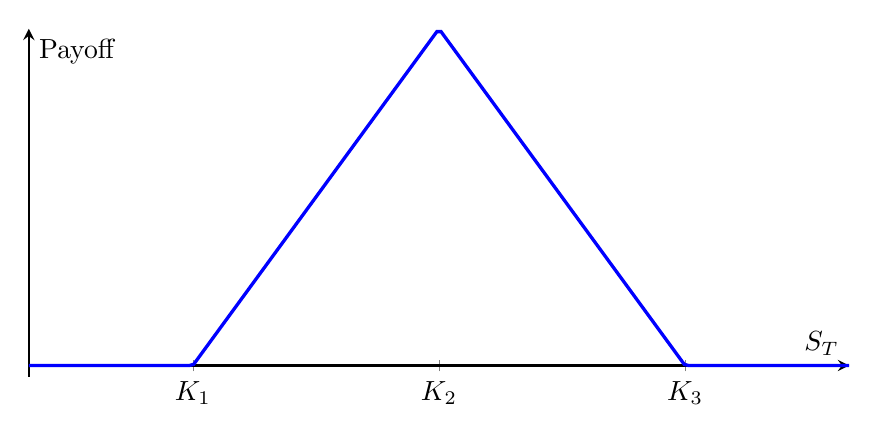
\begin{tikzpicture}
  \begin{axis}[
    axis x line=middle,
    axis y line=middle,
    xlabel={$S_T$},
    ylabel={Payoff},
    ymin=-1, ymax=30,
    xmin=50, xmax=150,
    xtick={70, 100, 130},
    xticklabels={$K_1$, $K_2$, $K_3$},
    ytick=\empty,
    domain=50:150,
    samples=200,
    width=12cm,
    height=6cm,
    thick
  ]
    \addplot[blue, very thick] 
      {max(x-70,0) - 2*max(x-100,0) + max(x-130,0)};
  \end{axis}
\end{tikzpicture}
\\
\small{\textit{Payoff du Call Butterfly Spread}}
\end{center}




% Le payoff en fonction de $S_T$ est de forme ``papillon'' :
% croissance linéaire entre $K_1$ et $K_2$, puis décroissance entre $K_2$ et $K_3$, nul ailleurs.

% \begin{center}
% \includegraphics[width=0.6\textwidth]{butterfly_payoff_example.pdf}
% \end{center}

% Cette stratégie constitue donc un \textbf{arbitrage pur} :
% on encaisse une prime initiale et le payoff est toujours non négatif.




\section{Put Spread}

\subsection*{Exercice :}

\begin{exerciseBox}[Put Spread]
On considère un sous-jacent $S$ et deux options put européennes de même maturité $T$ :  

 \begin{itemize}
     \item un put de strike $K + \varepsilon$, de prix $P_1 = 10$ ;  
    \item un put de strike $K$, de prix $P_2 = 11$.  
 \end{itemize}

On construit un \emph{put spread} en achetant le put de strike $K + \varepsilon$ et en vendant le put de strike $K$.  
\\
\textbf{Question} : \textit{y a-t-il une opportunité d’arbitrage ?}
\end{exerciseBox}



\subsection*{Solution :}


\textbf{Payoff du put spread :}
Le payoff d’un put de strike $K$ est $(K-S_T)^+$. Donc le payoff de la stratégie est
\[
\Pi_T \;=\; (K+\varepsilon - S_T)^+ \;-\; (K - S_T)^+ \;=\;
\begin{cases}
\varepsilon, & S_T < K,\\[3pt]
K+\varepsilon - S_T, & K \le S_T < K+\varepsilon,\\[3pt]
0, & S_T \ge K+\varepsilon.
\end{cases}
\]

% --- Tracé (optionnel) avec TikZ/pgfplots ---
\begin{center}
\begin{tikzpicture}
\begin{axis}[
  width=10cm, height=5cm,
  axis lines=middle,
  xlabel={$S_T$}, ylabel={$\Pi_T$},
  ymin=-0.2, ymax=1.2,
  xmin=0, xmax=2.6,
  xtick={0.8,1.8}, xticklabels={$K$, $K+\varepsilon$},
  ytick={0,1}, yticklabels={$0$, $\varepsilon$},
  domain=0:1.6, samples=2
]
% esp = 1 , k = 0.8 ,  
% palier à gauche: y = ε pour S_T < K
\addplot+[mark=none, domain=0:0.8] {1};
% segment décroissant entre K et K+ε : y = K+ε - S_T, mis à l'échelle
\addplot+[mark=none, domain=0.8:1.8] {1.8 - x};
% zéro à droite
\addplot+[mark=none, domain=1.8:2.6 , color=green] {0};

% points ouverts/fermés aux jonctions (pour le look)
\addplot[only marks, mark=*, mark size=1.8pt] coordinates {(0.8,1)};
\addplot[only marks, mark=*, mark size=1.8pt] coordinates {(1.8,0)};
\end{axis}
\end{tikzpicture}
\end{center}

\textbf{Le prix d'une option put européenne est croissant par rapport au strike }

Soit \( P(K) \) le prix, au temps \( t \), d'une option put de strike \( K \) et de maturité \( T \).
Sous la mesure risque-neutre, on a
\[
P(K) = e^{-r(T-t)} \, \mathbb{E}\big[ (K - S_T)_+ \,\big|\, \mathcal{F}_t \big].
\]
On dérive \( P(K) \) par rapport à \( K \) :
\[
\frac{\partial P}{\partial K}
= e^{-r(T-t)} \, \mathbb{E}\left[ 
\frac{\partial}{\partial K}(K - S_T)_+ \,\bigg|\, \mathcal{F}_t \right].
\]
Or, pour tout \( x \in \mathbb{R} \),
\[
\frac{\partial}{\partial K} (K - x)_+
= \mathbf{1}_{\{x < K\}},
\]
d'où
\[
\frac{\partial P}{\partial K}
= e^{-r(T-t)} \, \mathbb{E}\big[ \mathbf{1}_{\{S_T < K\}} \,\big|\, \mathcal{F}_t \big].
\]
En notant \( \mathbb{P}^t(\cdot) = \mathbb{P}(\cdot \mid \mathcal{F}_t) \), on obtient
\[
\frac{\partial P}{\partial K}
= e^{-r(T-t)} \, \mathbb{P}^t\big( S_T < K \big).
\]
Comme \( e^{-r(T-t)} > 0 \) et que la probabilité est toujours positive,
\[
\frac{\partial P}{\partial K} \ge 0.
\]
Ainsi, le prix d'une option put européenne est bien \textbf{croissant} par rapport au strike \( K \).


Donc, théoriquement  $P(K+\varepsilon) > P(K)$,Or, d'après l'énoncé, $P(K+\varepsilon) = 10$ et $P(K) = 11$,donc il y a une opportunité d'arbitrage.




\section{Parité call--put}

\subsection*{Exercice :}

\begin{exerciseBox}[Parité call--put]
On considère des options européennes (call $C_t(K,T)$ et put $P_t(K,T)$) de même strike $K$ et même maturité $T$,
écrites sur un sous-jacent $S_t$ ne versant pas de dividendes.
   

\medskip
\noindent
\textbf{Question.} Montrer la \emph{parité call--put} :
\[
C_t(K,T) - P_t(K,T) \;=\; S_t \;-\; K\,e^{-r(T-t)}.
\]

\end{exerciseBox}




\subsection*{Solution}

\textbf{Méthode 1 : Raisonnement d'arbitrage (réplication).}

Considérons deux portefeuilles :
\[
A := \begin{cases}
\text{long } 1 \text{ call } (K,T) \\
\text{long } K e^{-r(T-t)} \text{ d'obligation zéro-coupon}
\end{cases}
B :=  \begin{cases}
\text{long } 1 \text{ put } (K,T) \\
\text{long } 1 \text{ action } S
\end{cases}
\]
À l'échéance $T$, leurs payoffs valent
\begin{align*}
\Pi_T(A) &= (S_T - K)_+ + K \;=\; \max(S_T, K),\\
\Pi_T(B) &= (K - S_T)_+ + S_T \;=\; \max(S_T, K).
\end{align*}
Donc $\Pi_T(A)=\Pi_T(B)$ pour tout $S_T$. Par absence d'arbitrage, leurs valeurs aujourd'hui doivent coïncider :
\begin{align*}
C_t(K,T) + K e^{-r(T-t)} \;=\; P_t(K,T) + S_t
\;\;\Longleftrightarrow\;\;
C_t(K,T) - P_t(K,T) \;=\; S_t - K e^{-r(T-t)}.
\end{align*}

% \smallskip
% \noindent
% \textit{(Détection d'arbitrage en cas de violation.)}
% Si $C_t - P_t > S_t - K e^{-r(T-t)}$, alors le portefeuille $A$ est \emph{surévalué} par rapport à $B$ :
% on shorte $A$ et on achète $B$ pour encaisser un gain initial sans risque (les payoffs étant identiques à $T$).
% Le raisonnement s'inverse si $C_t - P_t < S_t - K e^{-r(T-t)}$.

\textbf{Méthode 2 : Par la mesure risque-neutre.}

Sous la mesure risque-neutre $\mathbb{Q}$,
\begin{align*}
C_t(K,T) &= e^{-r(T-t)}\,\mathbb{E}^{\mathbb{Q}}\!\big[(S_T - K)_+ \,\big|\, \mathcal{F}_t\big],\\
P_t(K,T) &= e^{-r(T-t)}\,\mathbb{E}^{\mathbb{Q}}\!\big[(K - S_T)_+ \,\big|\, \mathcal{F}_t\big].
\end{align*}
On utilise l'identité pointwise
\[
(S_T - K)_+ - (K - S_T)_+ = S_T - K,
\]
d’où
\begin{align*}
C_t(K,T) - P_t(K,T)
&= e^{-r(T-t)}\,\mathbb{E}^{\mathbb{Q}}\!\big[S_T - K \,\big|\, \mathcal{F}_t\big] \\
&= e^{-r(T-t)}\Big(\mathbb{E}^{\mathbb{Q}}[S_T \mid \mathcal{F}_t] - K\Big).
\end{align*}
Or, en absence de dividendes, $e^{-rt}S_t$ est une martingale sous $\mathbb{Q}$, donc
\[
\mathbb{E}^{\mathbb{Q}}[S_T \mid \mathcal{F}_t] = S_t\,e^{r(T-t)}.
\]
Par suite,
\begin{align*}
C_t(K,T) - P_t(K,T)
= e^{-r(T-t)}\big(S_t e^{r(T-t)} - K\big)
= S_t - K e^{-r(T-t)}.
\end{align*}

\paragraph{Remarque :}
Si le sous-jacent verse un dividende continu au taux $q$, on a :
\[
C_t - P_t \;=\; S_t\,e^{-q(T-t)} \;-\; K\,e^{-r(T-t)}.
\]


\section{contrat forward}

\subsection*{Exercice : }

\begin{exerciseBox}[Prix à terme (forward)]
On considère un contrat de \emph{forward} livrant 1 unité du sous-jacent $S$ à la date $T$.
On suppose d'abord que $S$ ne verse pas de dividendes, puis on traite le cas d'un
dividende continu au taux $q$. Le taux sans risque en capitalisation continue est $r$.

\medskip
\noindent
\textbf{Questions.}
\begin{enumerate}
  \item Déterminer le \emph{prix à terme} (ou \emph{forward price}) $F_{t,T}$.
  \item Donner la \emph{valeur} au temps $t$ d'un forward existant avec prix de livraison $K$.
\end{enumerate}    
\end{exerciseBox}

\subsection*{Solution :}

% Considérons deux portefeuilles :
% \[
% A := \begin{cases}
% \text{long } 1 \text{ action } S \\
% \text{short } K  \text{ zéro-coupon avec } K = F(t,T) \quad 
% \end{cases}
% B :=  \begin{cases}
% \text{long } 1 \text{ forward }  \\
% % \text{long } 1 \text{ action } S
% \end{cases}
% \]

% \textbf{à t = 0 :}
% \begin{itemize}
%     \item $V_A( t = 0) = S_t - F(t,T).e^{-r(T-t)}$
%     \item $V_B(t=0) = 0$ : parce qu'à $t=0$ dans le contrat forward on paye rien, c'est un contrat à terme.
% \end{itemize}


% \textbf{à t = T :}

% \begin{itemize}
%     \item $V_A( t = 0) = S_T - F(t,T)$
%     \item  $V_B(t=0) = S_T - F(t,T)$ : à $t=T$ on détine du sous-jacent mais on paye le prix du forward 
% \end{itemize}

% donc comme $V_A(t=T) = V_B(t=T)$ donc par abssance d'opppertuinte d'arbitrage on a : 

% \[
% V_A(t=0) = V_B(t=0) \Rightarrow F(t,T) = \frac{S_t}{B(t,T)} = S_te^{r(T-t)}
% \]

Considérons deux portefeuilles :
\[
A := 
\begin{cases}
\text{long } 1 \text{ action } S,\\
\text{short } 1 \text{ zéro-coupon de nominal } F(t,T) \text{ (échéance } T).
\end{cases}
\qquad
B := 
\begin{cases}
\text{long } 1 \text{ contrat forward }.
\end{cases}
\]

\textbf{À la date } $t$ :
\begin{itemize}
  \item $V_A(t) = S_t - F(t,T)\,B(t,T)$, \quad où $B(t,T)=e^{-r(T-t)}$ est le prix du zéro-coupon.
  \item $V_B(t) = 0$ \; (un forward s’échange sans coût initial).
\end{itemize}

\textbf{À la date } $T$ :
\begin{itemize}
  \item $V_A(T) = S_T - F(t,T)$.
  \item $V_B(T) = S_T - F(t,T)$ \; (on reçoit le sous-jacent et on paie le prix à terme).
\end{itemize}

\vspace{0.5cm}


Comme $V_A(T)=V_B(T)$ pour tout $S_T$, l’absence d’opportunité d’arbitrage impose
\[
V_A(t)=V_B(t)
\;\;\Longrightarrow\;\;
S_t - F(t,T)\,B(t,T) = 0
\;\;\Longrightarrow\;\;
F(t,T) = \frac{S_t}{B(t,T)} = S_t\,e^{r(T-t)}.
\]


% \paragraph{Portefeuille $A$.} 
% Long $1$ forward $(t,T)$ de prix à terme $F_{t,T}$ \emph{et} long $B(t,T)$ unités de zéro-coupon.
% \begin{align*}
% \text{Coût initial de $A$} \ &=\ B(t,T)\cdot 1, \\
% \text{Payoff à $T$ de $A$} \ &=\ (S_T - F_{t,T}) + 1 \cdot 1 \ =\ S_T - F_{t,T} + F_{t,T} \ =\ S_T.
% \end{align*}

% \paragraph{Portefeuille $B$.}
% Achat immédiat d'une unité de l'actif : long $1$ sous-jacent.
% \begin{align*}
% \text{Coût initial de $B$} \ &=\ S_t, \\
% \text{Payoff à $T$ de $B$} \ &=\ S_T.
% \end{align*}

% \paragraph{Conclusion par absence d'arbitrage.}
% Les deux portefeuilles ont \emph{exactement le même payoff} à l'échéance ($S_T$). 
% Donc leurs coûts initiaux doivent coïncider :
% \begin{align*}
% S_t \ =\ B(t,T)\cdot F_{t,T}
% \qquad \Longrightarrow \qquad
% \boxed{\; F_{t,T} \ =\ \dfrac{S_t}{B(t,T)} \;}
% \end{align*}
% En particulier, si le taux est constant en capitalisation continue $r$, alors 
% $B(t,T)=e^{-r(T-t)}$ et
% \[
% F_{t,T} \ =\ S_t\, e^{r(T-t)}.
% \]


% \paragraph{Méthode 1 : Raisonnement par arbitrage (cash-and-carry).}

% \textit{(a) Sans dividendes.)}
% Le coût de portage d'une unité de $S$ de $t$ à $T$ est $S_t e^{r(T-t)}$.
% Par absence d'arbitrage, vendre à terme ou porter le sous-jacent doit coûter pareil :
% \begin{align*}
% F_{t,T} \;=\; S_t\,e^{r(T-t)}.
% \end{align*}
% \emph{Tests d'arbitrage.}
% Si $F_{t,T} > S_t e^{r(T-t)}$ : \textsc{cash-and-carry} (acheter $S$, financer à $r$, vendre le forward).
% Si $F_{t,T} < S_t e^{r(T-t)}$ : \textsc{reverse cash-and-carry} (vendre $S$ à découvert, placer à $r$, acheter le forward).

% \smallskip
% \textit{(b) Avec dividende continu $q$.)}
% Porter l'actif de $t$ à $T$ tout en \emph{réinvestissant} les dividendes revient à payer aujourd'hui
% le \emph{prépaid forward} $S_t e^{-q(T-t)}$ puis capitaliser à $r$ :
% \begin{align*}
% F_{t,T} \;=\; \big(S_t e^{-q(T-t)}\big)\,e^{r(T-t)}
% \;=\; S_t\,e^{(r-q)(T-t)}.
% \end{align*}
% \textit{(c) Dividendes discrets déterministes $D_i$ aux dates $t_i\in(t,T]$.}
% \[
% F_{t,T} \;=\; \Big(S_t - \sum_{t_i\in(t,T]} D_i e^{-r(t_i-t)}\Big)\,e^{r(T-t)}.
% \]

\textbf{Méthode 2 : Sous la mesure risque-neutre.}

Sous $\mathbb{Q}$, sans dividendes, $e^{-rt}S_t$ est une martingale, donc
\begin{align*}
\mathbb{E}^{\mathbb{Q}}[S_T \mid \mathcal{F}_t] \;=\; S_t\,e^{r(T-t)}
\quad\Longrightarrow\quad
F_{t,T} \;=\; \mathbb{E}^{\mathbb{Q}}[S_T \mid \mathcal{F}_t]
\;=\; S_t\,e^{r(T-t)}.
\end{align*}
Avec un dividende continu $q$, la dynamique neutre au risque vérifie
$\tfrac{dS_t}{S_t}=(r-q)\,dt+\sigma\,dW_t$, d'où
\begin{align*}
\mathbb{E}^{\mathbb{Q}}[S_T \mid \mathcal{F}_t]
\;=\; S_t\,e^{(r-q)(T-t)}
\quad\Longrightarrow\quad
F_{t,T} \;=\; S_t\,e^{(r-q)(T-t)}.
\end{align*}

